\documentclass{article}
\usepackage{graphicx}
\usepackage{lscape}
\usepackage{pdflscape}
\usepackage{booktabs}
\usepackage{natbib}
\usepackage{pdfpages}
\usepackage[acronym, toc, nonumberlist]{glossaries}
\usepackage{url} 
% \usepackage[none]{hyphenat}

\makeglossaries
\newacronym{iot}{IoT}{Internet of Things}
\newacronym{coap}{CoAP}{The Constrained Application Protocol}
\newacronym{udp}{UDP}{User Datagram Protocol}
\newacronym{rest}{REST}{Representational State Transfer}
\newacronym{m2m}{M2M}{Machine-to-Machine}
\newacronym{rpi}{RPi}{Raspberry Pi}

\title{Feasibility Study}
\author{Thomas Scott}
\date{1st October 2018}

\begin{document}
	\pagenumbering{gobble}
	\maketitle
	\newpage
	\pagenumbering{arabic}

	\section{Title}

	CoAP based IoT data transfer from a Raspberry Pi to Cloud 

	\section{Learning Objectives}
	
	\begin{itemize}	
	\item Use knowledge, abilities and skills for further study and for a range of employment in areas related to scientific and technical computing.
	\item Interpret legislation appropriate to computer professionals and also be aware of relevant ethical issues and the role of professional bodies.
	\item Analyse, design, and implement algorithms using a range of appropriate languages and/or methodologies.
	\item Demonstrate an understanding of the characteristics and operation of various networking technologies and communication protocols.
	\item Conduct an investigation in usage and implementation of communication protocols.
	\item Identify and make use of current scholarly research in the field.
	\item Demonstrate effective communication, decision making and creative problem solving skills, and identify appropriate practices within a professional, legal and ethical framework.
	\end{itemize}

	\section{Project Background}

	The Internet Engineering Task Force (IETF) standardised the Constrained Application Protocol `CoAP' as RFC 7252 in 2014 —as a specialized web transfer protocol for constrained devices, constrained nodes and constrained networks in the Internet of Things ‘IoTs’. \citep{bormann2015constrained}
	
	\gls{coap} is a software protocol that enables simple constrained ``things'' such as low-power sensors and actuators to communicate interactively via the internet. 
	It runs on devices that support the \gls{udp} and implements a lightweight application layer that suited for low-power, low-memory devices. 
	
	The goal of CoAP is to allow constrained devices to connect and communicate with one another over the Web. It accomplishes this by implementing a subset of the \gls{rest} architecture and supporting \gls{m2m} features such as discovery, multicast support and asynchronous message exchanges.

	The \gls{iot} can be viewed as a large distributed network comprising of highly dynamic devices \citep{miorandi2012internet}. Small low powered ``smart'' devices can connect and communicate with one another. Some of these devices can contain or communicate with sensors that record real world data. This data can then be transmitted to other devices allowing them to trigger actions. In this way groups of smart devices can be used to improve day to day situations such as automated houses (thermostats and heating etc.), security and improved monitoring.

	The Raspberry Pi 3 Model B \citep{pi3model} is a credit card sized computer developed by the Raspberry Pi Foundation. This small device contains a 1.4GHz 64-bit processor, wireless LAN, Bluetooth, faster Ethernet, 40-pin GPIO header and 4 USB 2.0 ports. The \gls{rpi}'s ability to act as a GNU/Linux server and the interfacing services provided by its general purpose I/O pins make it a popular choice of hardware for \gls{iot} applications. \citep{kumar2016iot}

	Cloud computing platforms enable the storage of data and the execution of programs on a remote widely accessible server. The use of cloud computing platforms allow users to access information from a variety of different locations and  devices. With 48\% of the UK market considering their smartphone as the most important device for internet access \citep{ofcom2018} cloud platforms are a large part in providing services to users. Cloud platforms are often easier to scale, allowing the connection of more smart devices and therefore a larger connected network. This project will look at how \gls{coap} can be used to transmit data to a cloud platform using a \gls{rpi} as a smart device connected to a sensor.


	\section{Aims}
	The aim of this project is to investigate the implementation of CoAP technology and how to use CoAP to send data to the cloud.

	\section{Objectives}
	\begin{enumerate}
	\item Explore existing research into using CoAP technology to send sensor data to a cloud service.
	\item Identify ways in which sensor data can be transferred using CoAP.
	\item Investigate and choose a cloud computing platform to send sensor data to.
	\item Investigate the usage of CoAP over different transport layers. (UDP, TLS).
	\item Compare CoAP to similar protocols (MQTT) that data to the cloud.
	\item Implement a CoAP client on a Raspberry Pi which:
		\begin{enumerate}
			\item Connects to a sensor attached to the device
			\item Connects to the internet
			\item Can transmit data collected from the sensor to a cloud platform
		\end{enumerate}
	\end{enumerate}

	\section{Required Resources}
	\begin{itemize}
		\item Raspberry Pi 3
		\item Micro SD card
		\item Power cord
		\item Sensor
		\item Cloud Platform (To be selected as part of project)
	\end{itemize}
	
	\section{Notable dates}
	\begin{table}[h]
		\begin{tabular}{@{}llll@{}}
		\toprule
		Week & Starting & Requirement                 & Deadline      \\ \midrule
		4    & 15/10/18 & Feasibility Study submitted & 19/10/18      \\
		12   & 10/12/18 & Prototype Report uploaded   & 14/12/18      \\
		18   & 11/02/19 & Product submitted           & 22/02/19      \\
		20   & 25/02/19 & Report Outline uploaded     & 01/03/19      \\
		25   & 01/04/19 & Showcase held               & Specified day \\
		25   & 01/04/19 & Report submitted            & 05/04/19      \\ \bottomrule
		\end{tabular}
	\end{table}

	\begin{landscape}
		
		\section{Tasks and Timescale}
		
		\begin{figure}[ht]
			\centering
			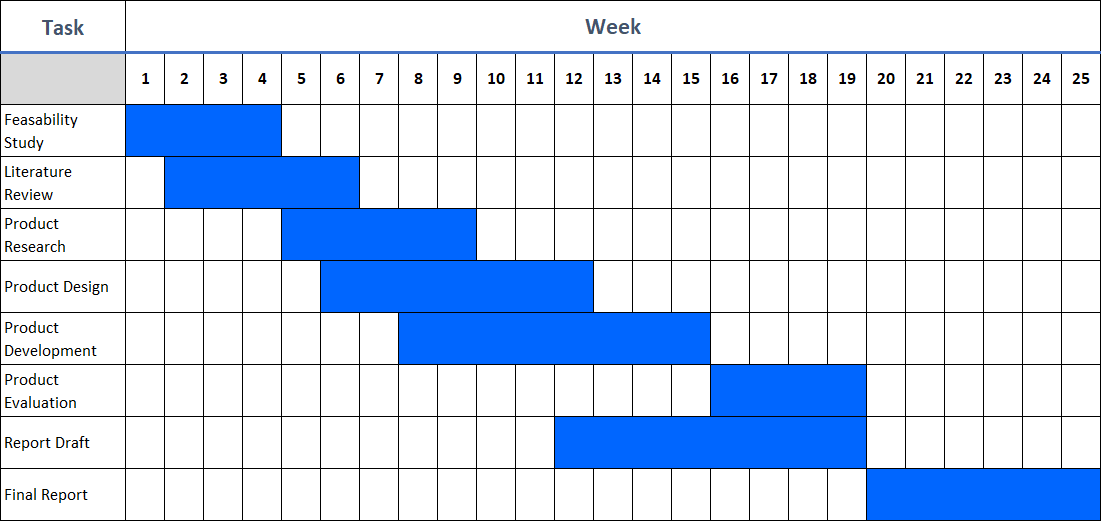
\includegraphics[width=\linewidth, height=\textheight,keepaspectratio]{gantt.png}
		\end{figure}

	\end{landscape}

	\printglossaries

	\bibliographystyle{agsm}
	\bibliography{references}

	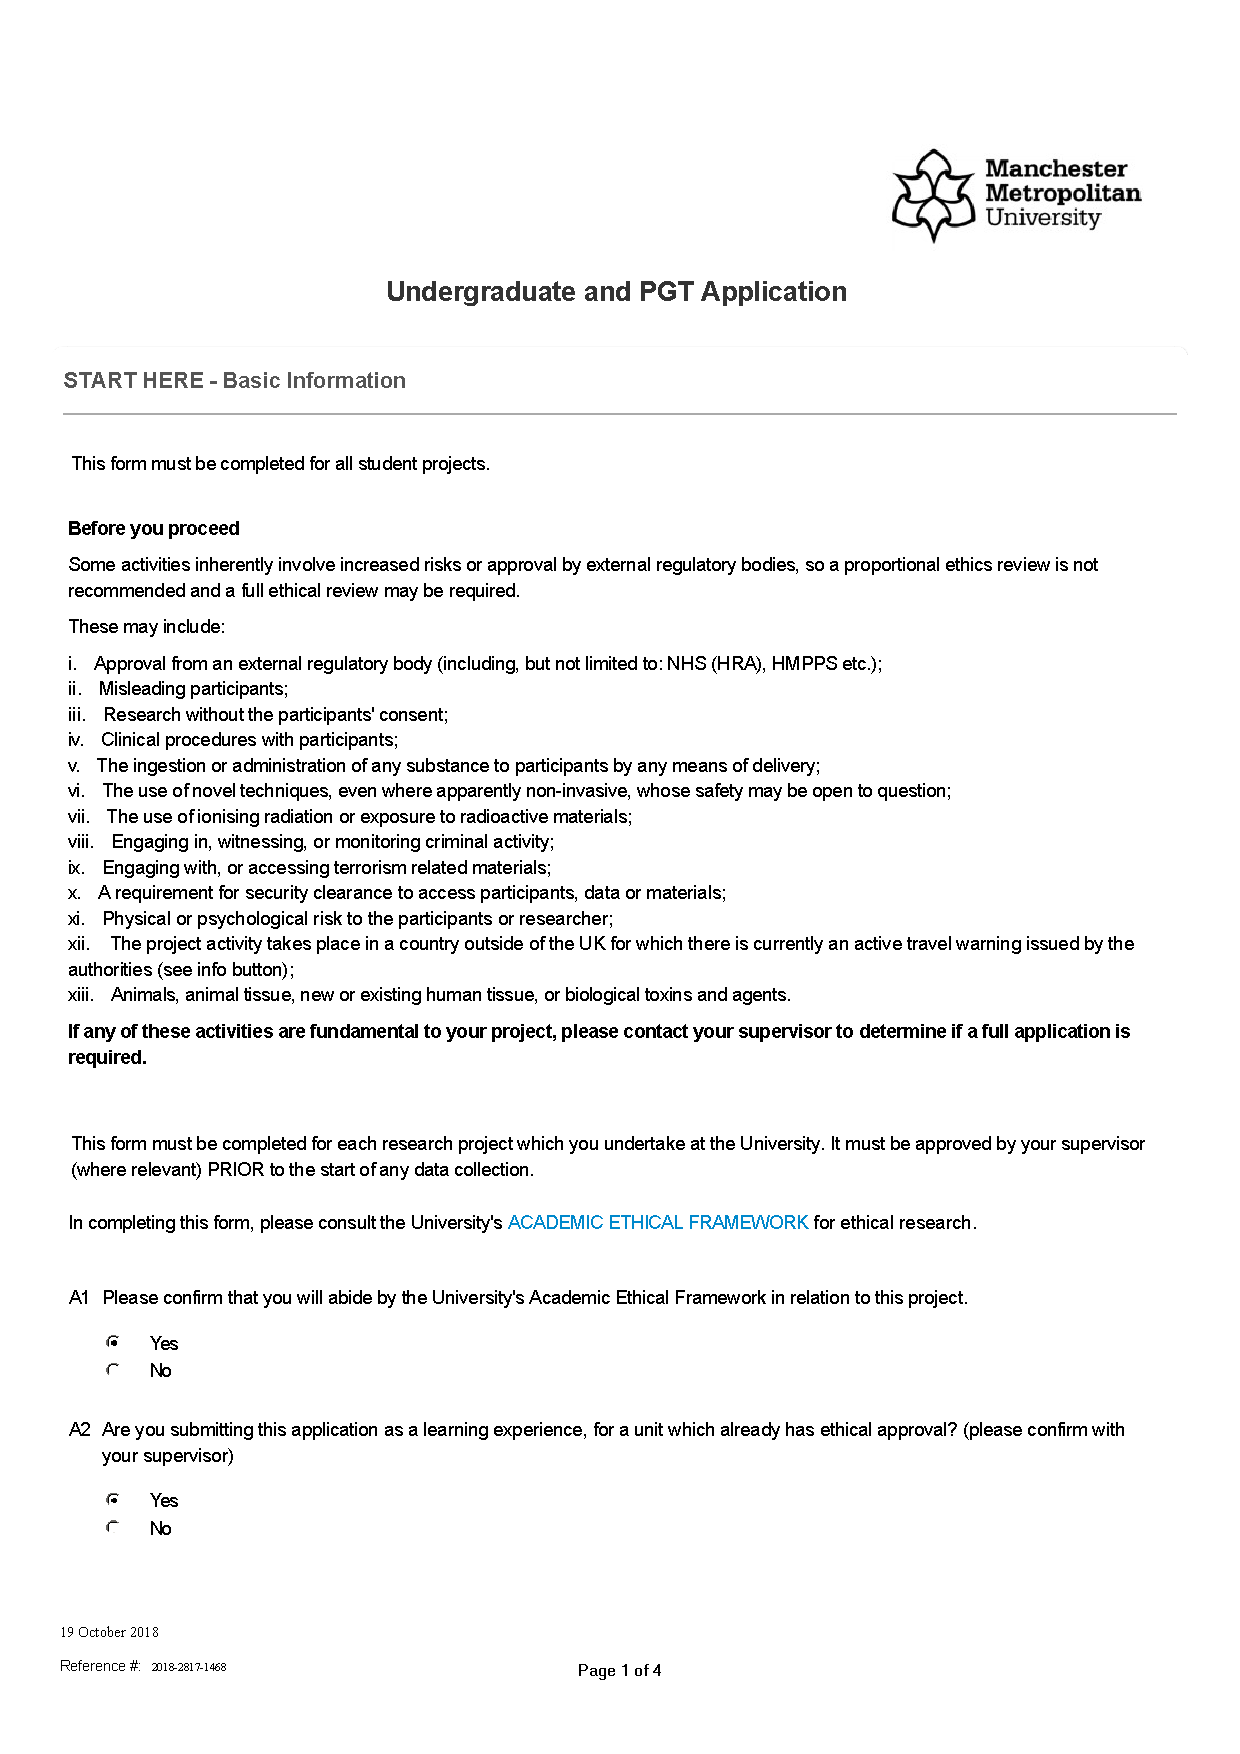
\includepdf[pages=-,pagecommand={}]{ethics_form.pdf}

	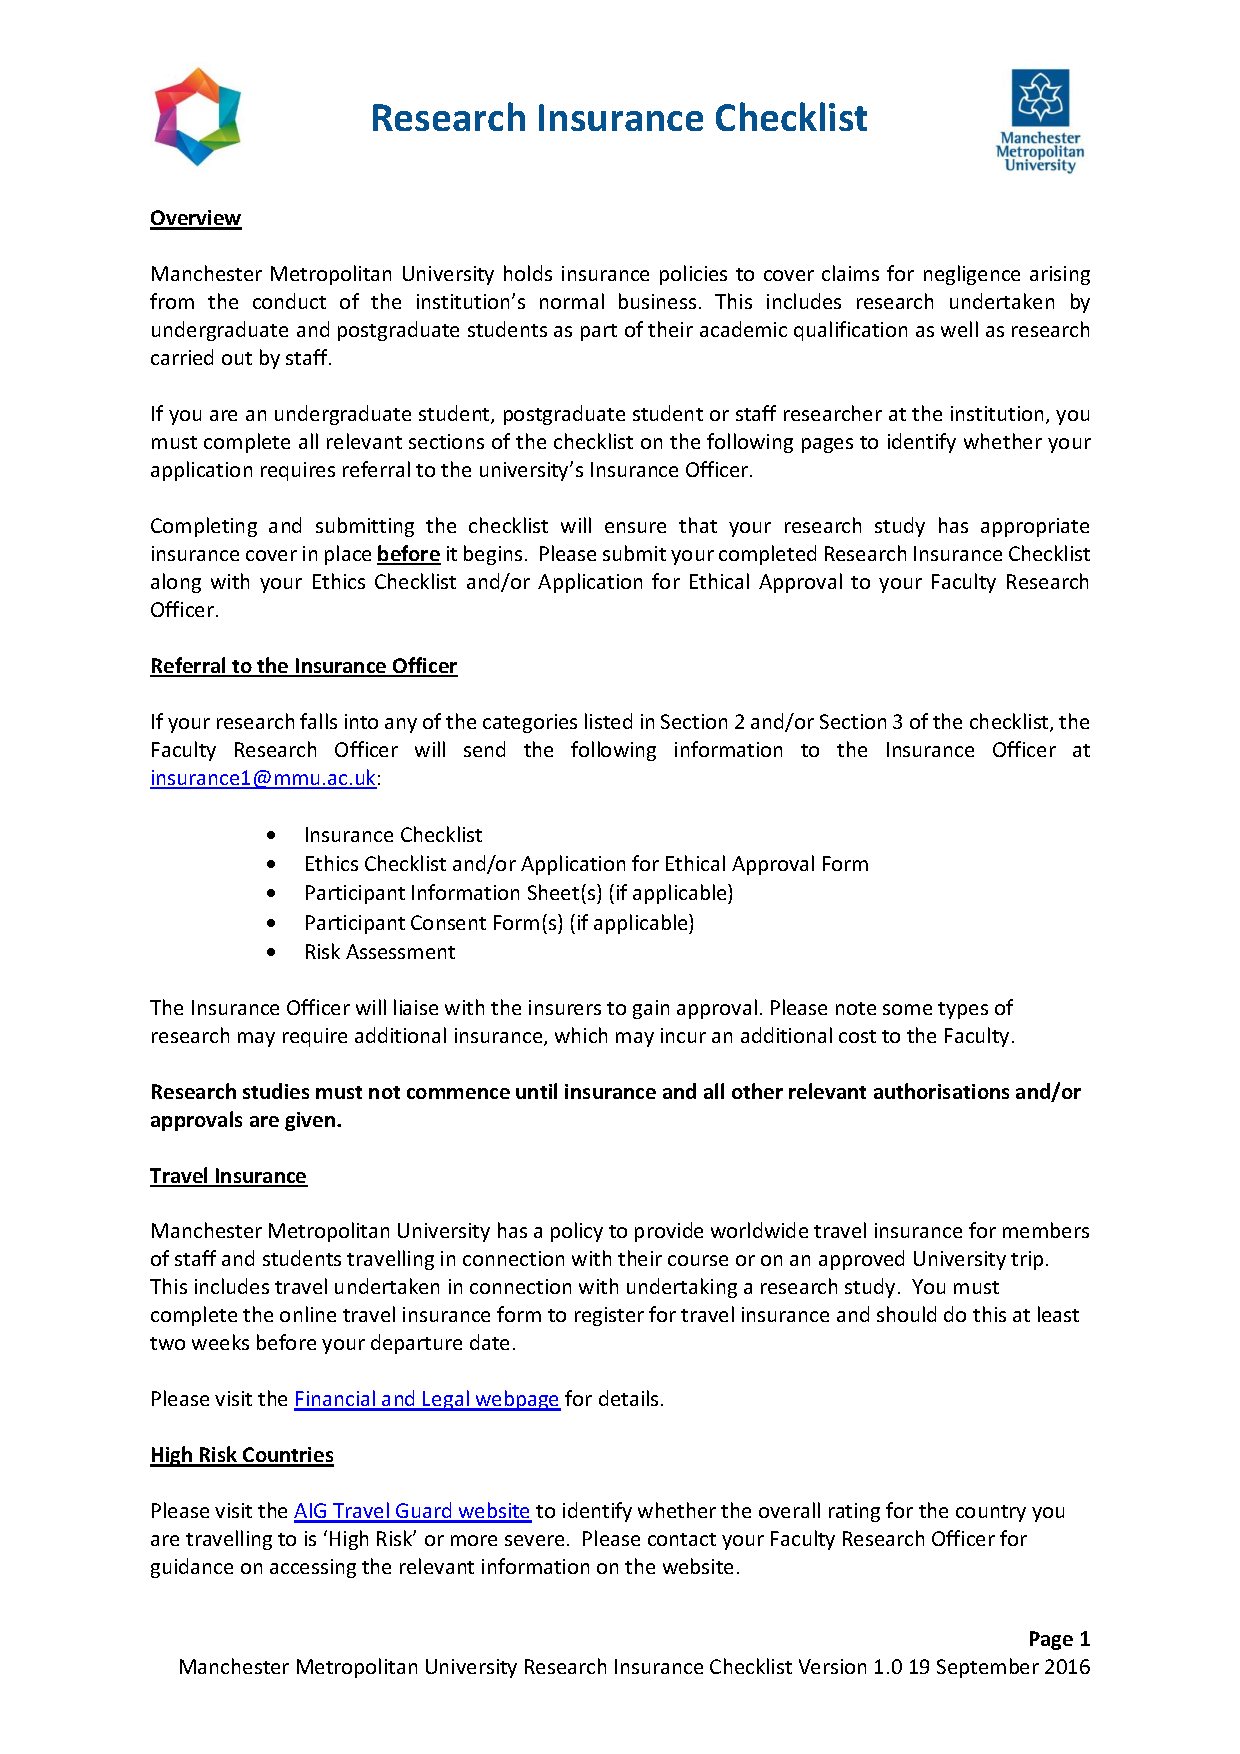
\includepdf[pages=-,pagecommand={}]{MMU-Research-Insurance-Checklist-v1-0-19-Sept-2016.pdf}

\end{document}

